% \begin{savequote}[75mm]
% Does this shit even work?
% \qauthor{A Tired Grad Student}
% \end{savequote}

\chapter{High-throughput behavior in rats}
\newthought{The laboratory rat \textit{Rattus norvegicus}} was the first mammalian species domesticated for scientific research\cite{Jacob1999}, and has since been the most widely studied species in biomedical research. Rats are not only experimentally tractable and straightforward to raise in captive, but moreover, they have a well-documented capacity for learning laboratory tasks. In psychology and neuroscience disciplines, rats have been the standard model for studying a range of cognitive capacities, including decision-making\cite{Raposo2012, Miller2017TwoStep, Piet2018, Brunton2013}, working memory\cite{Bratch2016, Fassihi2014, Akrami2018}, relational or associative memory\cite{Dusek1997, Abada2013ReversalDisease}, and spatial navigation\cite{OKeefe1971, Whishaw1995, Aronov2014, Poo2020}. 

One of the most widely used tools for studying animal behavior in the lab is the operant conditioning chamber. With the operant conditioning chamber, the experimenter gradually shapes the animal's behavior with positive or negative feedback until the animal regularly produces (or refrains from) a given behavior. Most rodent behavior experiments rely on operant conditioning, and technological developments over the past ten years have enabled experimenters to use computer-controlled systems that allow for automated and high-throughput training of many animals in parallel. 

Automated training methods are more efficient as they require little to no hands-on involvement from the experimenter. Animals can be placed into chambers by staff who may be less biased about the particular study's goals or they can simply live in the boxes with automatically or remotely controlled training regimes\cite{Qiao2018, Miller2017TwoStep, Poddar2013}. Thus, high-throughput systems not only allow for more systematic and less biased experiments, but also allow many animals to be trained and studied in parallel. Higher-throughput studies provide statistical power difficult to achieve with small-scale animal cohorts and importantly, have the potential to provide a readily available source of animals for physiological access or perturbation studies. These advantages are particularly important for behavioral tasks that are complex and require long training schedules.

Several groups have demonstrated the power of high-throughput training systems for the study of cognitive behaviors in rats. Of note, Brody and colleagues use highly complex tasks that take rats anywhere from 1 month to 4-6 months to learn\cite{Brunton2013, Miller2017TwoStep, Constantinople2019} and have developed high-throughput, automated training systems that train many rats in parallel (20 to 30+ rats\cite{Brunton2013, Constantinople2019} on various decision-making and working memory tasks\cite{Miller2017TwoStep, Brunton2013}. In motor skill learning, {\"O}lveczky and colleagues have built high-throughput, fully-automated systems for home-cage training, which allows similar ranges of animals to be trained in parallel on the same or different variants of a motor skill-learning task\cite{Poddar2013}. 

In the context of visual behaviors, rats have been studied for their capacity to discriminate shapes for a long time. In 1930, Karl Lashley\cite{Lashley1930} described a wide range of visual behaviors in rats. He trained rats to select one of two visual stimuli in order to access one hidden door, behind which there was a food reward\cite{Lashley1938}. Using this classic two-choice paradigm, Lashley demonstrated that rats are capable of a range of shape discriminations. Prusky developed a water version of the two-choice task that leverages rats' natural swimming abilities, and used this paradigm to measure visual acuity in rats and mice, finding that rats had superior visual acuity\cite{Prusky2000}. Over the last ten years, a growing number of studies have demonstrated rats' ability to perform tasks of invariant or tolerant object recognition using a similar two-choice paradigm as Lashley's hidden doors and Prusky's two-arm water maze\cite{Zoccolan2009, Vermaercke2012, Tafazoli2012, Alemi-Neissi2013, Djurdjevic2018}. While most studies in monkeys rely on about 2-3 animals, standard rat vision studies use $~$4-6 animals per experiment. Inspired by the work of Brody, {\"O}lveczky, and others, our goal was to take existing visual behavior paradigms in rats and adapt them for high-throughput, automated training. 

% %%%%%%%%%%%%%%%%%%%%%%%%%%%%%%%%%%%%%%%%%%%%%%%%%%%%%%%%%
% Results
% %%%%%%%%%%%%%%%%%%%%%%%%%%%%%%%%%%%%%%%%%%%%%%%%%%%%%%%%%
% fig:openratbox
% fig:basic_training
% fig:behavior_generalization

% ---------------------------------------------------------
% OpenRatBox -- the hardware.
% ---------------------------------------------------------
\section{OpenRatBox: An open-source platform for high-throughput visual behavior experiments in rats}
My approach was to design a system that was reproducible, low-cost, and modular. It was critical to design training boxes that would be straightforward to reproduce, not only to maintain constancy from one box to the next, but also to facilitate widespread use both within the lab and across labs. Systematization across research groups can be immensely powerful, especially for studying highly complex, multi-modal processes like decision-making, as exemplified by the International Brain Laboratory and the Allen Brain Institute.

% FIGURE 1.1 OpenRatBox Schematic
\begin{figure}[t!]
    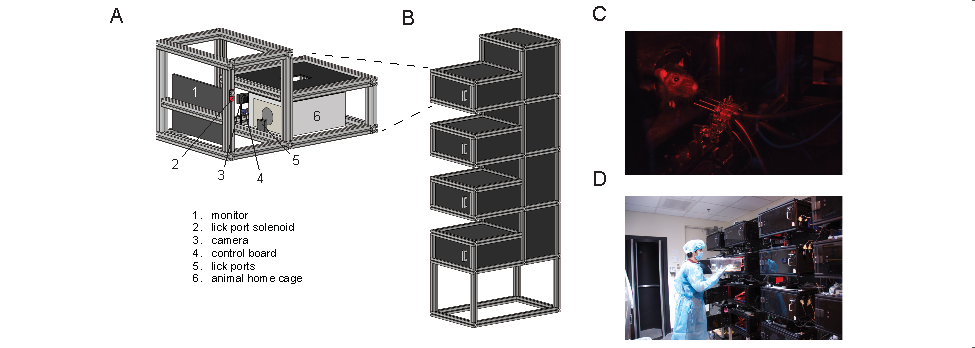
\includegraphics[width=\textwidth]{figures/chapter_1/fig_1-1_openratbox/fig_1-1_openratbox_compressed.pdf}
    \vspace{.1in}
    \caption[OpenRatBox]{OpenRatBox: Open-source, automated, high-throughput training. \textbf{A.} Schematic of one training box. Numbers denote relevant parts. 
    \textbf{B.} Left, A full tower assembly of four identical training boxes. \textbf{C.} A photograph of a rat in a training box equipped for a three-port task. \textbf{D.} A photograph of a room of towers used to train the animals in the present work. An experimenter is shown loading an animal in its home cage into the training box.  
    \label{fig:openratbox}}
\end{figure}

In order to build behavior boxes at a larger scale, I relied on low-cost, readily accessible components and open-source software for experimental control. While it is possible to build a highly sophisticated and customized apparatus that meets the particular demands of a given experiment, it can be extremely costly and hard to adapt for other experiments or impossible to use by other labs. In contrast, designing a low-cost system that relies on open-source technology allows it to be more accessible as a tool that can benefit others, while also allowing for continued improvements and new adaptations. 

Modularity is important because a given behavior can be tested under different regimes. For example, two commonly used behavior choice paradigms are Go/No-Go and two-alternative forced choice (2AFC) tasks, which offer different advantages and disadvantages (see \cite{Bjerre2020} for a recent review). At the hardware level, while Go/No-Go paradigms only require a single reward port or choice manipulandum, 2AFC and other multi-choice tasks require at least two. The use of a single response can be slightly less complicated and take less time to learn, but Go/No-Go paradigms can result in over-reporting or ambiguity about No-Go responses (for example, it can be ambiguous whether the animal fails to respond because it is not motivated, does not understand the task, or is correctly withholding a response)\cite{Andermann2010, Petreanu2012, Guo2014ProceduresMice}. On the other hand, two different responses help to clarify some ambiguity as the animal must respond one way or another, depending on what is presented\cite{OConnor2010, Zhong2019}. However, these paradigms, by virtue of being more complicated, can take longer to learn (weeks as opposed to days)\cite{Mayrhofer2013, Guo2014ProceduresMice}. Though I tested both Go/No-Go and two-choice behavior paradigms, I focus on the latter for the remainder of this chapter as this is a well-established paradigm used to test visual object recognition behavior in rats\cite{Lashley1930, Zoccolan2009, Prusky2000}.

Each training box is designed to be identical, and experiment-specific adjustments could be made with modular components. The main vestibule of each unit houses the animal's cage and all hardware needed to collect the animal's response and monitor its behaviors (Figure\ref{fig:openratbox}A). Each unit is equipped with a small computer that allows as many experiments to be run independently and in parallel as there are boxes. The external frame is composed of aluminum extrusion bars and custom-cut acrylic paneling that fits into the railing slots of the bars, such that an arbitrary number of boxes can be built on top of the next, limited by the available vertical space, and any number of additional hardware items can be mounted directly to the rack. In our behavior rooms, we had enough space for towers composed of 4 stacked units (Figure\ref{fig:openratbox}B). 

Within a given unit, there are two partitions (Figure\ref{fig:openratbox}A). The monitor is mounted on a partition separate from the main vestibule in order to keep it clean and protected (for example, from chewing, or stray water droplets and bedding). The animal has visual access to the monitor through a window separating the monitor from the main vestibule that holds the cage. Specifically, the animal extrudes its head out a small hole placed in the window. Mini extrusion bars are screwed directly into the acrylic floor of the main vestibule around the animal's access hold. This effectively creates a mountable rail system for attaching experiment-specific components, such as reward ports, USB cameras, and IR detectors. As such, any modifications specific to a paradigm (\textit{e.g.}, one reward port or three reward ports, see example in Figure\ref{fig:openratbox}C) could be easily attached or removed from one box to the next. 

All wiring feeds through small access holes cut into the acrylic pieces embedded into the extrusion bars, as does tubing for water delivery of rewards. Attached to each box is a small computer (MacMini, due to their compact size, though others are possible) that runs the experiment (visual stimulation, I/O control, and so on). Finally, all the training boxes are controlled and monitored by a control computer running a client (MWorks) that interfaces with the servers running in each behavior box. 
 
The cage itself is held in place with two spring-loaded latches that allow the cage to be loaded into the same relative position, if necessary. The cage locking mechanism was adapted from a commercially available, self-standing animal cage rack, in which each cage is locked into the air circulation and filtration system. The box is thus designed to support fully live-in animal behavior training. If transporting animals between daily sessions, the experimenter need only to load the animal into a training cage and slip the cage into the box (Figure\ref{fig:openratbox}D). In the case of live-in training, the animal's access window can be gated shut during non-training times, if desired.

In addition to specific behavior task constraints, such as single or multiple reward ports, a desirable feature of behavior systems is the ability to combine them with physiology or neural manipulations. The behavior rigs are modular enough that rats with tethered cables can also be housed in the boxes, as there is sufficient room for an access port and a commutator that can hold the cabling attached to the animal's head. Thus, the entire system can be equipped for neural stimulation and recording in tethered rats. The spacing between the stacked boxes can be kept as is or adjusted for a commutator system that carries a cable from the animal's head through a hole in the acrylic ceiling of the main vestibule. 

% ---------------------------------------------------------
% OpenRatBox -- the functionality (high-throughput training)
% ---------------------------------------------------------
\section{High-throughput behavior training}
We first trained rats to perform a simple, two-category object discrimination task\cite{Zoccolan2009} (Figure\ref{fig:basic_training}A). This is a two-choice task in which the rat navigates between three different ports to start trials and provide responses. Specifically, the rat licks a center port to initiate a trial, which triggers an image to appear on computer monitor. The rat indicates which object the image corresponds to be licking one of the two flanking ports, \textit{e.g.}, the left port, for object A, and the other \textit{e.g.}, for object B (Figure\ref{fig:basic_training}B).

% FIGURE 1.1 Basic training
\begin{figure}[t!]
    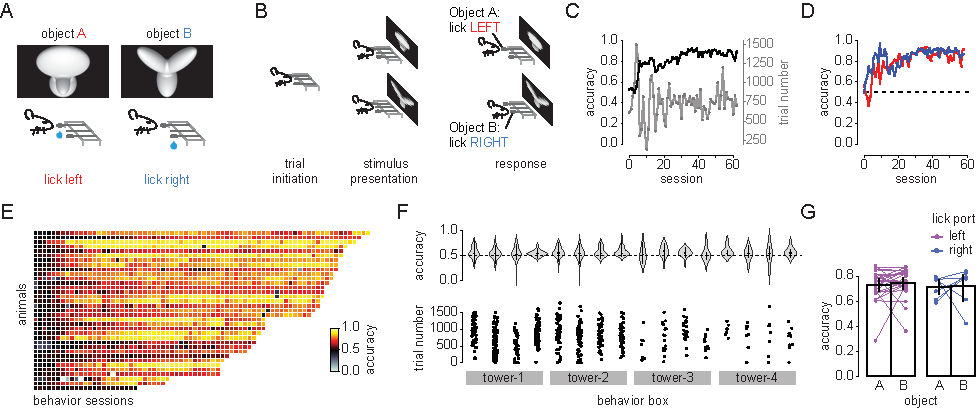
\includegraphics[width=\textwidth]{figures/chapter_1/fig_1-2_basic_training/fig_1-2_basic_training.pdf}
    \vspace{.1in}
    \caption[High-throughput training]{High-throughput training on a simple two-alternative choice task. 
    \textbf{A.} Logic of the basic, two-category object discrimination task. 
    \textbf{B.} Trial structure (adapted from \cite{Zoccolan2009}). Rats initiate a trial by licking the center port. After a variable delay, an image appears on the screen. The animal licks the left or right port to indicate it sees object A or object B (or vice versa). Correct responses result in water rewards, while incorrect responses result in negative feedback (see Methods). 
    \textbf{C.} Example training data for one rat. Black, overall accuracy by training session. Gray, number of trials completed in each session. 
    \textbf{D.} Accuracy in \textbf{C} split by object identity. Colors correspond to each of the two object identities.
    \textbf{E.} Training accuracy by session number for a large cohort of animals (N=29 out 32 rats reached criterion performance of 70\% accuracy). 
    \textbf{F.} \textit{Top}: Accuracy for each box and tower. 4 boxes were vertically stacked to create 1 tower, 4 towers are shown (indicated by gray boxes below the plots, tower-1, tower-2, \textit{etc.}). The relative position of each group within the tower represents the same physical location in each tower (top, second from the top, \textit{etc.}). \textit{Bottom}: Number of trials performed per session in each box and tower during training. Each dot denotes a session for an animal. Organization of grouped points is the same as the upper panel (corresponding to boxes and towers). 
    \textbf{G.} Performance split by stimulus-port mapping and object identity. REFREF, accuracy for object A. REFREF, accuracy for object B. Port numbers 1 and 2 denote whether the animal is assigned to lick port 1 for object A or port 2 for object A, and vice versa.
    \label{fig:basic_training}}
\end{figure}

Animals could be trained to perform shape discriminations in one month or less, and readily performed several hundreds of trials per day in the automated training rig (Figure\ref{fig:basic_training}C-D). Importantly, overall behavior metrics were similar across all behavior box units and towers. We observed no differences in overall accuracy or number of trials completed per session (Figure\ref{fig:basic_training}E-F). One disadvantage of two-choice tasks is that animals can tend to form response biases. Although there were biases across rats (see Supplemental Figure\ref{supfig:heatmaps}, our automated training protocol was successful in correcting response biases, and most animals showed high accuracy levels for each of the two objects (Figure\ref{fig:basic_training}D, G). 

Across multiple cohorts of rats trained to discriminate two objects (see Methods, Phase 1 of Training), training results were highly reproducible and consistent (n=48/56 rats reached criterion performance of 70\% correct across 12.6 +/- 7.6 s.d. sessions, see Supplemental Figure\ref{supfig:aggregate_training}). These results demonstrate that our behavior units are reproducible and successful for training large cohorts of animals. 

% ---------------------------------------------------------
% Behavior Generalization
% ---------------------------------------------------------
\section{Visual object recognition behavior}
Once rats were trained to perform basic two-choice discriminations, there were many permutations of shape comparisons to be studied. Previous studies have demonstrated that rats are capable of recognizing never-before-seen views of familiar objects\cite{Zoccolan2009, Vermaercke2012, Tafazoli2012}, and the high-throughput training system I designed was inspired by the desire to make these questions more easily studied in rats. The rats successfully discriminated between the two, highly-trained images. Thus, the next step was to test whether rats will perform more complex visual object recognition behaviors in OpenRatBox. Specifically, we sought to test two types of generalizations previously shown to be robust in rats\cite{Zoccolan2009, Tafazoli2012}: the first was a perceptual similarity test of the two original objects, by which we identified rats’ discrimination thresholds separating one object from another, and the second was an invariant recognition test, with which we evaluated rats' ability to recognize the objects across changes in particular view (Figure\ref{fig:behavior_generalization}A). 

% FIGURE 1.3 Behavior generalization.
\begin{figure}[t!]
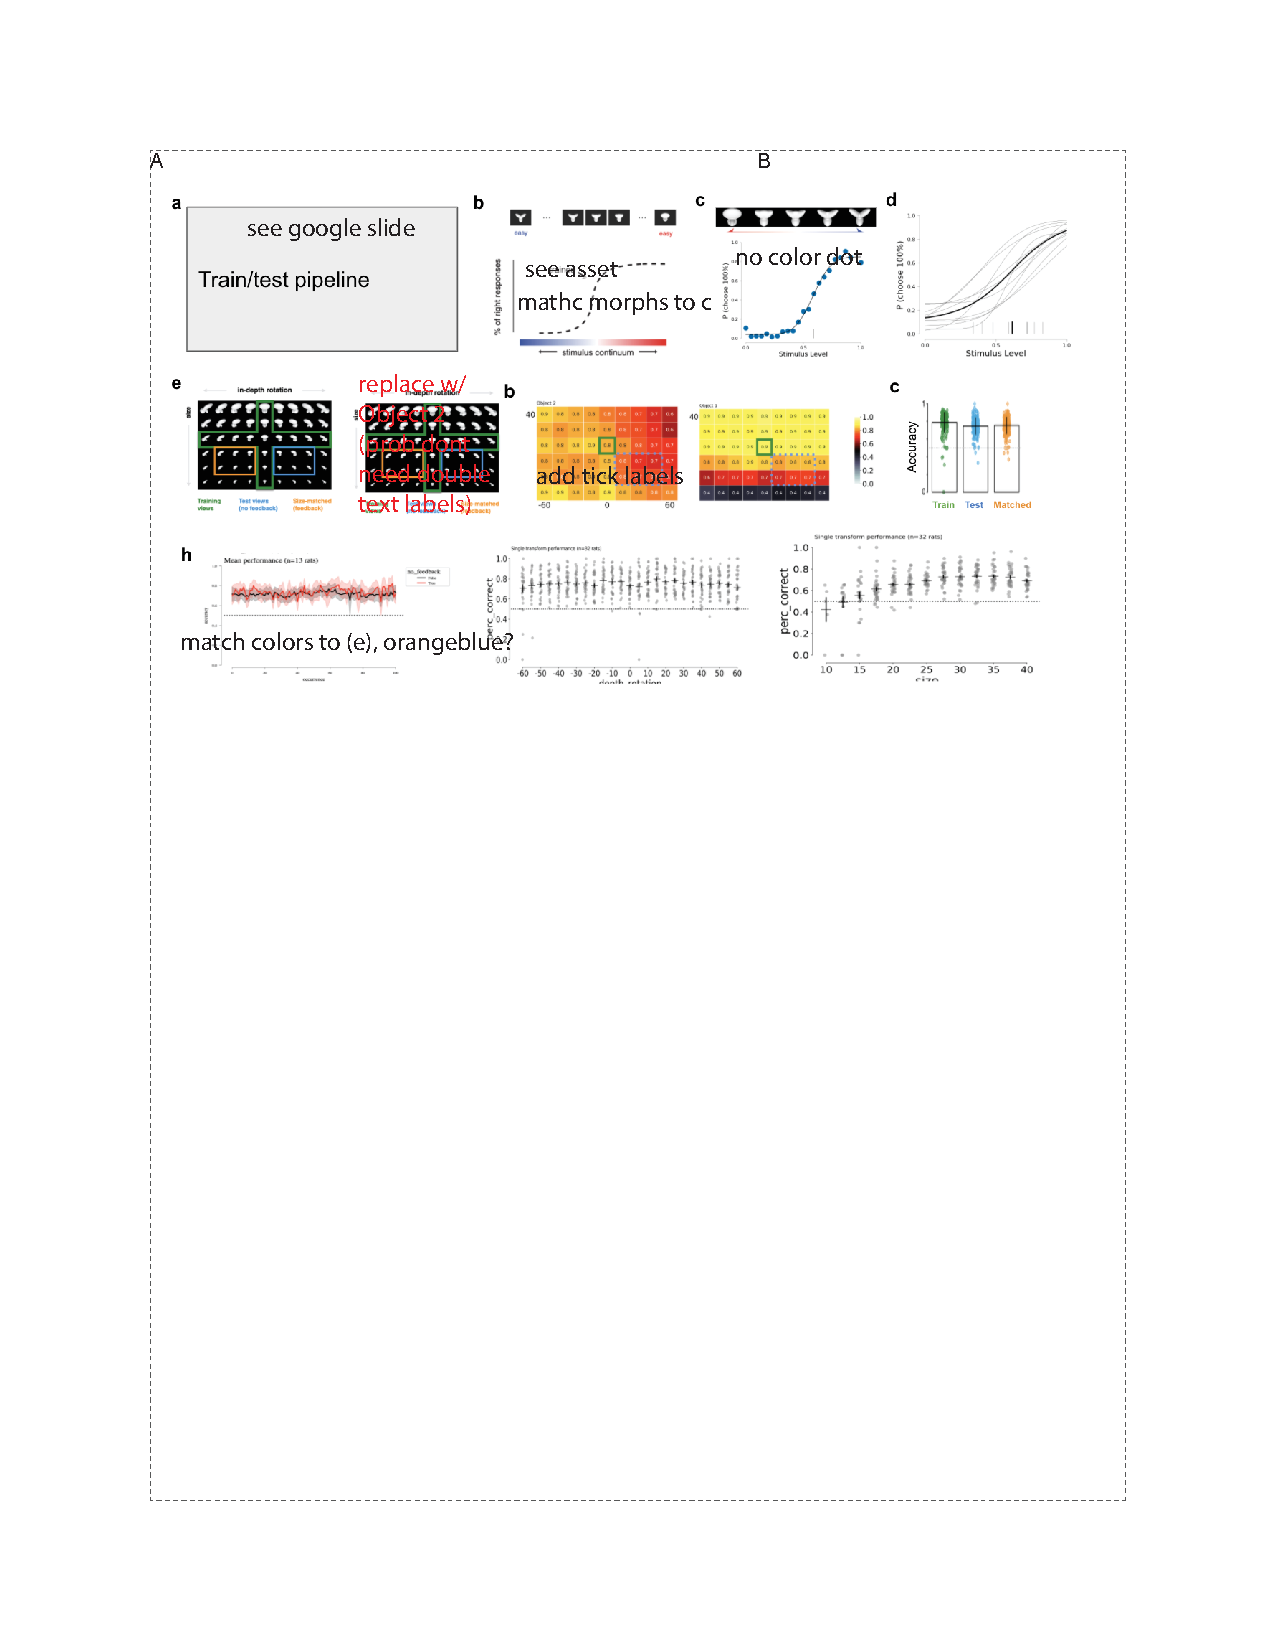
\includegraphics[width=\textwidth]{figures/chapter_1/fig_1-3_behavior_generalization/fig_1-3_behavior_generalization.pdf}
    \vspace{.1in}
    \caption[Generalization of visual behavior]{Generalization to identity-preserving and identity-changing transformations. 
    \textbf{A.} Training and testing pipeline. Animals are first trained on the basic discrimination task. Those that pass criterion performance are then tested on identity-changing or identity-preserving generalizations on probe trials that are interleaved with the basic task. 
    \textbf{B.} Morph stimuli create an axis along which identity changes across a stimulus continuum between the original anchors, object A and B. 
    \textbf{C.} Example data on the morph probe trials for one rat. Dots, average across trials for each morph level. Line, fit psychometric curve. 
    \textbf{D.} Psychometric curves for one cohort (N=10 of 13 rats that passed criterion on the anchor objects, see Methods). Thin lines, individual rats. Thick line, average psychometric curve across rats. 
    \textbf{E.} Identity-preserving transformations tested for each of the original objects: 6 sizes and 9 in-depth rotations. Green, subset of conditions used for training. Green, test transformations for which feedback was never provided. Purple, size-matched, \textit{i.e.}, acuity-matched, transformations of the test views, but for which feedback was provided, to compare the effect of feedback on generalization performance. No-feedback quadrants were counterbalanced across animals. 
    \textbf{F.} Performance for all identity-preserving transformations for each object for an example rat. Colors and stimulus conditions are ordered as in \textbf{E}. \textbf{G.} Accuracy for rats in one cohort (n=10 rats) for train views, test views, and size-matched feedback views. Colors as in \textbf{E}. Each circle denotes session accuracies for a given rat, all rats shown. Error bars, SD.
    \textbf{H.} Accuracy as a function of the Nth presentation of a given transformation for feedback-provided (purple) and no-feedback (green) conditions. Shading, SD across animals. Dashed line, 50\% accuracy, or chance performance.
    \textbf{I.} Accuracy for each depth-rotation tested. Each dot is the session accuracy for a given rat. Horizontal and vertical bars, mean and SD across sessions. Dashed line, chance performance.
    \textbf{J.} Same as \textbf{I}, but for each stimulus size tested. Conventions as in \textbf{I}.
    \label{fig:behavior_generalization}}
\end{figure}

% paragraph about stimuli
The two original objects were recreated from a previous study by Zoccolan \textit{et al.}\cite{Zoccolan2009} that demonstrated invariant object recognition behavior using a computer-controlled training system in a small cohort of rats. The stimuli were created to reduce the animal's ability to perform generalizations based on purely low-level properties, \textit{e.g.}, luminance, as these properties, though they do vary across objects, are not diagnostic of object identity, since they also vary with changes in view for the same object. To address these concerns, the goal was to ensure that differences between views of any one object (within-object difference) were greater than the differences between the two objects at a particular view (between-object difference) (see Supplemental Figure\ref{supfig:stimulus_metrics}A). Moreover, when creating the axis along which the object identity changed, or morphed, from one anchor to the other, this relationship should hold, with within-morph differences across views being larger than between-morph differences at a given view (see Supplemental Figure\ref{supfig:stimulus_metrics}C-D).

Only rats that reliably discriminated between the two original objects (minimum 70\% accuracy on the basic two-choice task) were tested on generalization capacity. To identify perceptual discrimination thresholds, we presented the rats with identity-changing transformations in which images parametrically varied between the two original objects at a given view. Specifically, I created a shape continuum by generating a series of morphs that varied along a high-dimensional identity axis separating the two original objects (Figure\ref{fig:behavior_generalization}B). The identity axis was defined in N-dimensional pixel space, and morphs were selected to evenly sample distances along this axis (see Methods). The axis ranged from morph level 0, defined as 0\%B, to morph level 100 (or 1, if expressed as fractions), defined as 100\%B. We then tested the extent to which linear similarity in pixel space reflected perceived similarity in rats trained to discriminate the two anchor objects. 
Rats were presented with an intermediate morph image on a small fraction of trials (<15\%, see Methods) during the ordinary discrimination task. No feedback was provided on these probe trials in order to measure perceived, rather than trained, perceptual judgements. These probe trials were then used to build a psychometric curve to determine the animals' naive behavior in classifying the images as corresponding more to object A or object B. Curves were fit to the probe trials using maximum likelihood estimation (see Methods). These curves characterize the category boundary along the morph axis (Figure\ref{fig:behavior_generalization}B). I found that that rats perceptual choices matched the physical similarity of the morphed objects, though there was individual variation across  rats(Figure\ref{fig:behavior_generalization}C-D). Perceived similarity across the morph axis was centered around the true 50\% level, though slightly biased toward object B (threshold: 0.61 +/- 0.17, just-noticeable-difference, JND: 0.34 +/- 0.10, mean +- SD across n=10 rats, see Methods). 

% FIGURE 1.3 INVARIANCE TEST
To test how well animals discriminate objects across shape changes that preserve object identity, we tested the trained rats on the invariant object recognition task in which rats trained to discriminate object A and object B had to generalize performance across novel views of A and B (Figure\ref{fig:behavior_generalization}E). Following previously published methods, rats that passed criterion performance on the basic task (default view of object versus default view of object B0) were gradually introduced to a more complex version of two-choice task over several training phases (see Methods). Briefly, rats started with presentations in which the anchor objects changed over a single transformation, either size or rotation (grey cross in Figure\ref{fig:behavior_generalization}E). Once they demonstrated stable performance with the limited set of novel views, all the other combinations of size and rotation were introduced. 

In theory, each rat could memorize the correct response to every single image (\textit{i.e.}, view) of each object, which would not reflect the true generalization capacity of being able to spontaneously recognize an object in the real-world --- we are able to recognize something, like our keys, in places or contexts we have never seen them in before. To address this concern, each rat was assigned a subset of views (Figure\ref{fig:behavior_generalization}E, purple box) for which they never received feedback, like the morph probes. As an additional control, a subset of other views matched in size (\textit{i.e.}. acuity-matched) to the no-feedback views served to evaluate generalization performance --- if performance on the no-feedback views was low, comparing performance on size-matched conditions could disambiguate whether this was due to poor generalization or just those particular conditions being more difficult (because they were smaller).


Consistent with previous studies\cite{Zoccolan2009}, we found that performance generalized robustly across identity-preserving transformations along stimulus size and in-depth rotation (Figure\ref{fig:behavior_generalization}F-G). Importantly, accuracy was high on test trials (~80\% accuracy), where animals never received feedback (Figure\ref{fig:behavior_generalization}F-G), demonstrating that performance on novel views was spontaneous, rather than learned. In fact, accuracy was high across all presentations of novel views, with or without feedback (Figure\ref{fig:behavior_generalization}H). Although there was variability across animals in accuracy for each of the transformation axes of rotation and size (Figure\ref{fig:behavior_generalization}I-J), all rats showed high accuracy across all views. The only exception in the results presented here was low accuracy for the smallest stimulus size tested (Figure\ref{fig:behavior_generalization}J). However, when we tested a separate cohort of animals (data not shown) that were only presented with the smallest stimulus sizes, rats showed high levels of performance, suggesting this is a strategy effect, rather than a reflection of rats' inability to perform the task. These results demonstrate that rats are capable of true generalization, and are not simply learning stimulus-response pairings. 

% ---------------------------------------------------------
% Closing remarks
% ---------------------------------------------------------

\section{Concluding Remarks}
% summary
In summary, I describe a high-throughput behavior system, OpenRatBox, that robustly and reliably trains large cohorts of rats to perform visual tasks (Figure\ref{fig:openratbox}). Rats readily perform hundreds of trials per day, and training is consistent across all replications of the training box, demonstrating that the training unit is both reliable and reproducible (Figure\ref{fig:basic_training}). I then use OpenRatBox to show that rats robustly generalize to novel views of objects in a complex visual behavior task that requires the animals to make perceptual choices about more than two highly-trained images. Specifically, I tested rats' ability to generalize performance across identity-preserving transformations, and to make perceptual choices that follow our morph axis of identity transformations (Figure\ref{fig:behavior_generalization}). Although similar behavioral results have been shown previously\cite{Zoccolan2009, Tafazoli2012, Vermaercke2012}, the results presented here demonstrate that a) we can replicate these results in a high-throughput behavior system that allows an unparalleled number of rats to be trained on visual object recognition tasks, and b) in response to our particular stimuli, rats respond appropriately in the absence of training on the particular views (no feedback conditions and morph probe trials). These behavioral responses were important for selecting a stimulus set for characterizing neural representations of complex objects in rat visual cortex, which is addressed in Chapter 4. 

% some bonus features/future-directions-y
Several additional features designed into OpenRatBox promise to provide broader benefits to the community of researchers studying rat behavior. First, the training box is modular, allowing multiple reward port configurations, as well as combination with neural recording and manipulation. Specifically, both single-port (Go/No Go) and multi-port (2AFC) tasks can be tested by swapping out the port array screwed into the micro-frame in front of the animal's cage. For neural recording and/or stimulation, a hole cut into the top panel of the training box allowed wiring to connect from a headstage affixed to the animal's head to a commutator mounted just outside the box to offset the weight carried by the animal and prevent the tether from tangling. Second, the training system is low-cost, relying on relatively inexpensive components and open-source software (Arduino, MWorks, OpenEphys). All of the custom-cut paneling and parts are also available in a publicly accessible repository (see Supplemental Materials), allowing either the exact same system to be built or custom modifications for future experiments. 

% comparison to what has existed
A major goal of this collection of studies is to establish a robust pipeline for high-throughput behavior and cellular resolution imaging in awake rats. Due to the difficulty of the visual behaviors under study (weeks of training), and the inevitable attrition rate when physiology that comes when trying to perform neural recordings in the context of learned tasks, a training system that outputs large numbers of animals with minimal experimenter intervention is highly valuable. Groups that study cognitively-demanding tasks in rats that take months to train have demonstrated the power of high-throughput systems, both in sheer animal throughput (30-40+ rats in some cases\cite{Brunton2013, Constantinople2019}, as well as the ability to then partition subsets of trained animals for neural perturbations or recordings\cite{Erlich2011, Hanks2015, Constantinople2019}. In contrast, most visual object recognition studies in rats rely on much smaller cohorts of about 10 rats, though typically, much fewer at about 5-6 rats\cite{Zoccolan2009, Tafazoli2012, Vermaercke2012, Alemi-Neissi2013, Vinken2017}. As a low-cost and open-source system that is highly reproducible, OpenRatBox provides more traditional rat vision experiments with the high-throughput training capacity that has proven immensely powerful for studies that specifically use rats for their capacities in other cognitive behaviors, such as decision-making or working memory.

% Next steps
% Combining behavior with electrophysiology recordings or neural perturbations is relatively standard procedure for many studies of cognitive behavior in rats. Specifically for visual behaviors, head-fixing animals is critical for precise stimulus delivery and retinal monitoring.





% In Go/No-Go (GNG) paradigms, the animal responds to a given stimulus (the "Go" condition) by licking a choice port or pressing a lever, and must withhold a response otherwise (the "No-Go" condition). GNG paradigms have fewer moving parts, requiring only one response type, which can make it easier to learn. However, subjects tend to make more Go responses in the GNG task, as the Go response is rewarded while other other behaviors are not\cite{REFREF}. 

% For physiology experiments, GNG paradigms are more amenable to head-restrained animals, since the animal only needs to make one type of response. On the other hand, since reward strongly modulates neural activity, and GNG paradigms can be challenging as the stimulus, response, and reward are tightly linked\cite{REFREF}. Multi-port tasks, like two-choice paradigms, overcome many of these drawbacks, as the animal is trained to respond in one way to condition A and some other way to condition B. In this way, the stimulus, response, and reward can be disentangled, but at the cost of a more complicated task structure that can make interpretations difficult in still other ways. However, they can be more difficult to adapt for head-restrained conditions. Animals normally use head movements or their whole body to reach one reward port or the other\cite{REFREF}, which is not possible in physiology experiments that require the animal's head to be fixed in place in the recording apparatus. 


% \texttt{This is a line of code.}


% For an example of a full page figure, see Fig.~\ref{fig:myFullPageFigure}.

% % EXAMPLE FIGURE 
% \begin{figure}[t!]
%     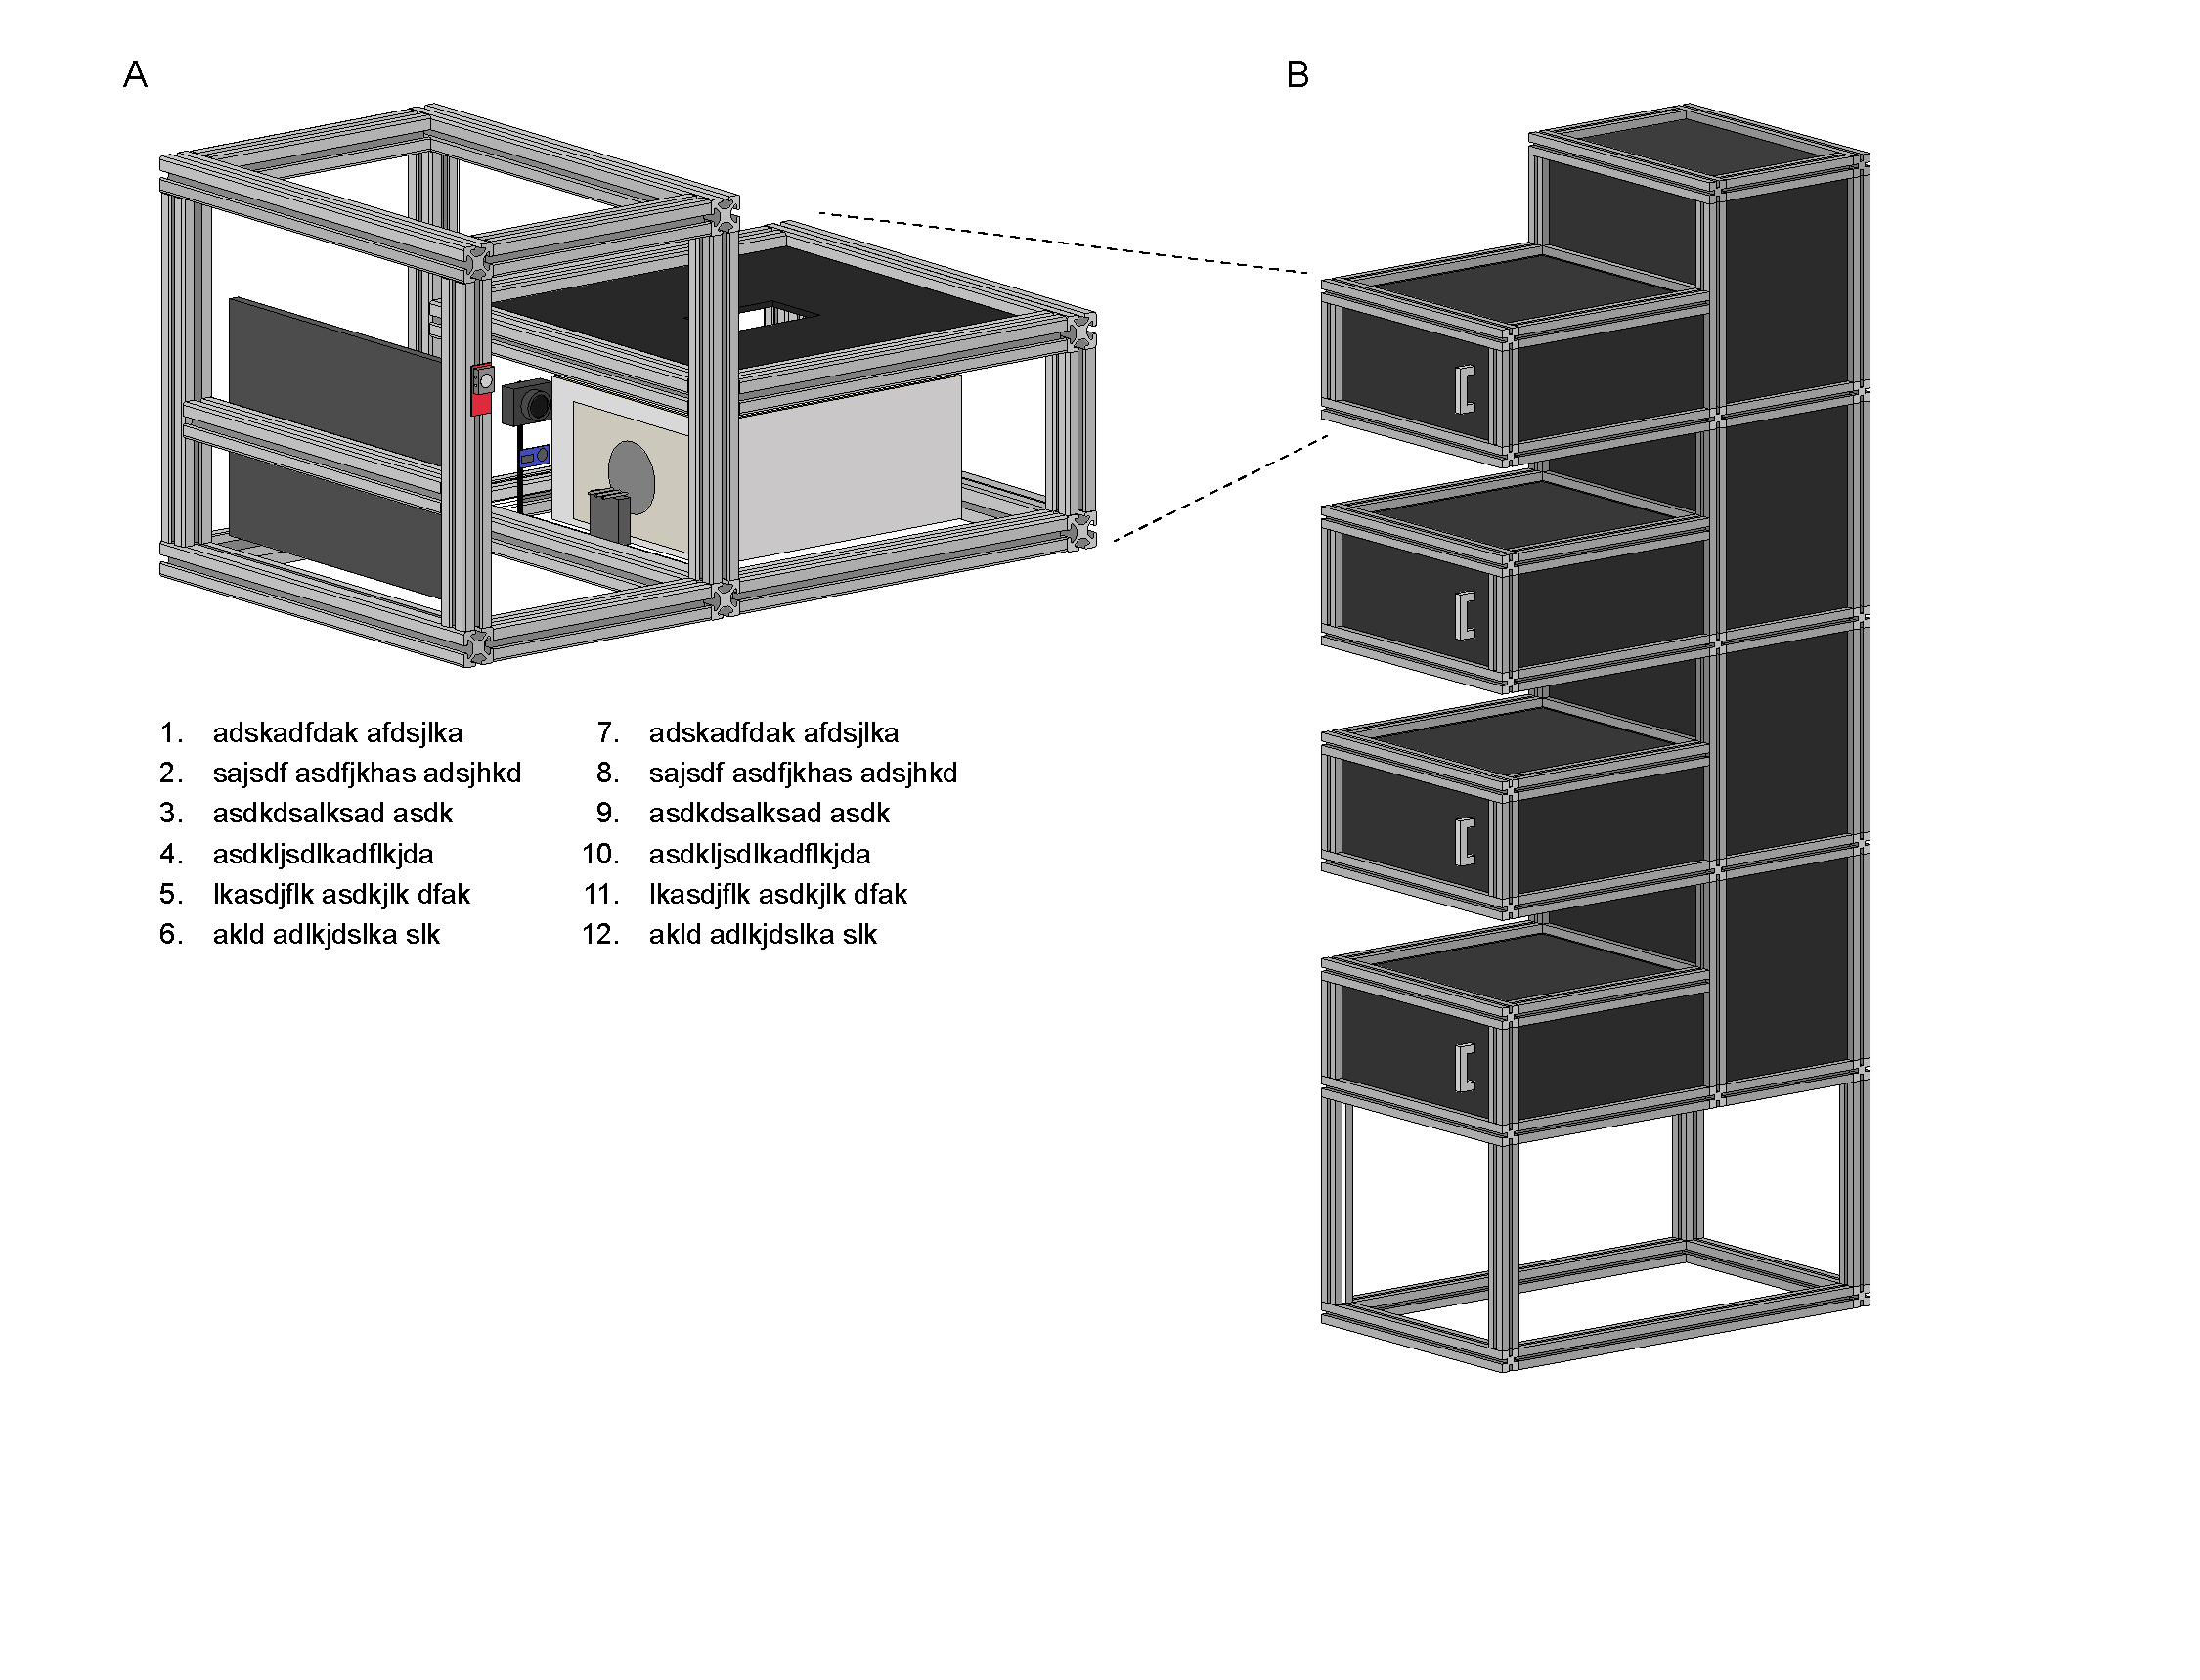
\includegraphics[width=\textwidth]{figures/chapter_1/ratbox_schematic.pdf}
%     \vspace{.1in}
%     \caption*{\textbf{Figure 2.1} Example figure and tips -- A) Your figure numbers should follow the format of Figure chapter#.figure#. B) Set width equal to textwidth. C) Specify position as [t!] to insert at page top.}
% \end{figure}

%% Requires fltpage2 package
%%
% \begin{FPfigure}
% 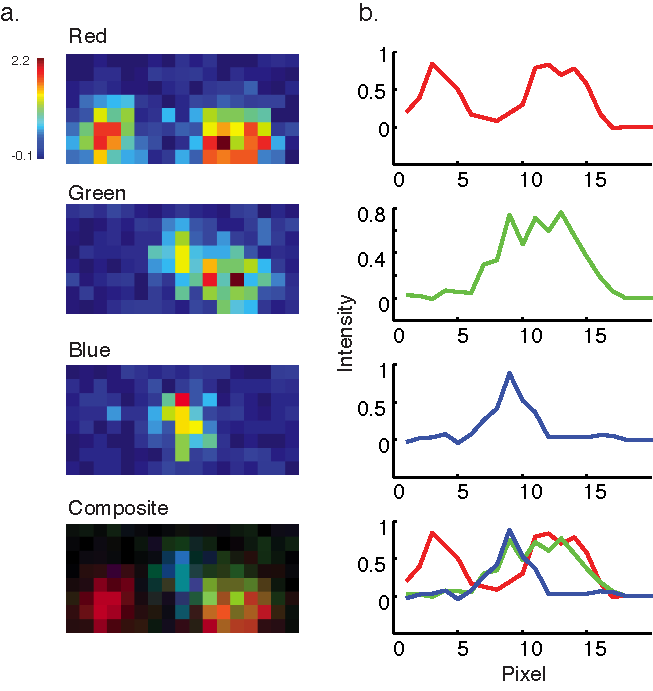
\includegraphics[width=\textwidth]{figures/fullpage}
% \caption[Short figure name.]{This is a full page figure using the FPfigure command. It takes up the whole page and the caption appears on the preceding page. Its useful for large figures. Harvard's rules about full page figures are tricky, but you don't have to worry about it because we took care of it for you. For example, the full figure is supposed to have a title in the same style as the caption but without the actual caption. The caption is supposed to appear alone on the preceding page with no other text. You do't have to worry about any of that. We have modified the fltpage package to make it work. This is a lengthy caption and it clearly would not fit on the same page as the figure. Note that you should only use the FPfigure command in instances where the figure really is too large. If the figure is small enough to fit by the caption than it does not produce the desired effect. Good luck with your thesis. I have to keep writing this to make the caption really long. LaTex is a lot of fun. You will enjoy working with it. Good luck on your post doctoral life! I am looking forward to mine. \label{fig:myFullPageFigure}}
% \end{FPfigure}
% \afterpage{\clearpage}

